% Options for packages loaded elsewhere
\PassOptionsToPackage{unicode}{hyperref}
\PassOptionsToPackage{hyphens}{url}
%
\documentclass[
  english,
  man,floatsintext]{apa6}
\usepackage{lmodern}
\usepackage{amsmath}
\usepackage{ifxetex,ifluatex}
\ifnum 0\ifxetex 1\fi\ifluatex 1\fi=0 % if pdftex
  \usepackage[T1]{fontenc}
  \usepackage[utf8]{inputenc}
  \usepackage{textcomp} % provide euro and other symbols
  \usepackage{amssymb}
\else % if luatex or xetex
  \usepackage{unicode-math}
  \defaultfontfeatures{Scale=MatchLowercase}
  \defaultfontfeatures[\rmfamily]{Ligatures=TeX,Scale=1}
\fi
% Use upquote if available, for straight quotes in verbatim environments
\IfFileExists{upquote.sty}{\usepackage{upquote}}{}
\IfFileExists{microtype.sty}{% use microtype if available
  \usepackage[]{microtype}
  \UseMicrotypeSet[protrusion]{basicmath} % disable protrusion for tt fonts
}{}
\makeatletter
\@ifundefined{KOMAClassName}{% if non-KOMA class
  \IfFileExists{parskip.sty}{%
    \usepackage{parskip}
  }{% else
    \setlength{\parindent}{0pt}
    \setlength{\parskip}{6pt plus 2pt minus 1pt}}
}{% if KOMA class
  \KOMAoptions{parskip=half}}
\makeatother
\usepackage{xcolor}
\IfFileExists{xurl.sty}{\usepackage{xurl}}{} % add URL line breaks if available
\IfFileExists{bookmark.sty}{\usepackage{bookmark}}{\usepackage{hyperref}}
\hypersetup{
  pdftitle={EDLD 651 Final Project: Discriminatory Experiences, Chronic Strain, Social Connectedness, and Psychological Wellbeing Among Individuals With Marginalized Sexual Orientations},
  pdfauthor={Maggie Head1, Sarah Spafford1, \& Heather Terral1},
  pdflang={en-EN},
  pdfkeywords={keywords},
  hidelinks,
  pdfcreator={LaTeX via pandoc}}
\urlstyle{same} % disable monospaced font for URLs
\usepackage{longtable,booktabs}
% Correct order of tables after \paragraph or \subparagraph
\usepackage{etoolbox}
\makeatletter
\patchcmd\longtable{\par}{\if@noskipsec\mbox{}\fi\par}{}{}
\makeatother
% Allow footnotes in longtable head/foot
\IfFileExists{footnotehyper.sty}{\usepackage{footnotehyper}}{\usepackage{footnote}}
\makesavenoteenv{longtable}
\usepackage{graphicx}
\makeatletter
\def\maxwidth{\ifdim\Gin@nat@width>\linewidth\linewidth\else\Gin@nat@width\fi}
\def\maxheight{\ifdim\Gin@nat@height>\textheight\textheight\else\Gin@nat@height\fi}
\makeatother
% Scale images if necessary, so that they will not overflow the page
% margins by default, and it is still possible to overwrite the defaults
% using explicit options in \includegraphics[width, height, ...]{}
\setkeys{Gin}{width=\maxwidth,height=\maxheight,keepaspectratio}
% Set default figure placement to htbp
\makeatletter
\def\fps@figure{htbp}
\makeatother
\setlength{\emergencystretch}{3em} % prevent overfull lines
\providecommand{\tightlist}{%
  \setlength{\itemsep}{0pt}\setlength{\parskip}{0pt}}
\setcounter{secnumdepth}{-\maxdimen} % remove section numbering
% Make \paragraph and \subparagraph free-standing
\ifx\paragraph\undefined\else
  \let\oldparagraph\paragraph
  \renewcommand{\paragraph}[1]{\oldparagraph{#1}\mbox{}}
\fi
\ifx\subparagraph\undefined\else
  \let\oldsubparagraph\subparagraph
  \renewcommand{\subparagraph}[1]{\oldsubparagraph{#1}\mbox{}}
\fi
% Manuscript styling
\usepackage{upgreek}
\captionsetup{font=singlespacing,justification=justified}

% Table formatting
\usepackage{longtable}
\usepackage{lscape}
% \usepackage[counterclockwise]{rotating}   % Landscape page setup for large tables
\usepackage{multirow}		% Table styling
\usepackage{tabularx}		% Control Column width
\usepackage[flushleft]{threeparttable}	% Allows for three part tables with a specified notes section
\usepackage{threeparttablex}            % Lets threeparttable work with longtable

% Create new environments so endfloat can handle them
% \newenvironment{ltable}
%   {\begin{landscape}\begin{center}\begin{threeparttable}}
%   {\end{threeparttable}\end{center}\end{landscape}}
\newenvironment{lltable}{\begin{landscape}\begin{center}\begin{ThreePartTable}}{\end{ThreePartTable}\end{center}\end{landscape}}

% Enables adjusting longtable caption width to table width
% Solution found at http://golatex.de/longtable-mit-caption-so-breit-wie-die-tabelle-t15767.html
\makeatletter
\newcommand\LastLTentrywidth{1em}
\newlength\longtablewidth
\setlength{\longtablewidth}{1in}
\newcommand{\getlongtablewidth}{\begingroup \ifcsname LT@\roman{LT@tables}\endcsname \global\longtablewidth=0pt \renewcommand{\LT@entry}[2]{\global\advance\longtablewidth by ##2\relax\gdef\LastLTentrywidth{##2}}\@nameuse{LT@\roman{LT@tables}} \fi \endgroup}

% \setlength{\parindent}{0.5in}
% \setlength{\parskip}{0pt plus 0pt minus 0pt}

% \usepackage{etoolbox}
\makeatletter
\patchcmd{\HyOrg@maketitle}
  {\section{\normalfont\normalsize\abstractname}}
  {\section*{\normalfont\normalsize\abstractname}}
  {}{\typeout{Failed to patch abstract.}}
\patchcmd{\HyOrg@maketitle}
  {\section{\protect\normalfont{\@title}}}
  {\section*{\protect\normalfont{\@title}}}
  {}{\typeout{Failed to patch title.}}
\makeatother
\shorttitle{EDLD 651 Final Project}
\keywords{keywords\newline\indent Word count: X}
\usepackage{csquotes}
\ifxetex
  % Load polyglossia as late as possible: uses bidi with RTL langages (e.g. Hebrew, Arabic)
  \usepackage{polyglossia}
  \setmainlanguage[]{english}
\else
  \usepackage[shorthands=off,main=english]{babel}
\fi
\ifluatex
  \usepackage{selnolig}  % disable illegal ligatures
\fi
\newlength{\cslhangindent}
\setlength{\cslhangindent}{1.5em}
\newlength{\csllabelwidth}
\setlength{\csllabelwidth}{3em}
\newenvironment{CSLReferences}[3] % #1 hanging-ident, #2 entry spacing
 {% don't indent paragraphs
  \setlength{\parindent}{0pt}
  % turn on hanging indent if param 1 is 1
  \ifodd #1 \everypar{\setlength{\hangindent}{\cslhangindent}}\ignorespaces\fi
  % set entry spacing
  \ifnum #2 > 0
  \setlength{\parskip}{#2\baselineskip}
  \fi
 }%
 {}
\usepackage{calc} % for \widthof, \maxof
\newcommand{\CSLBlock}[1]{#1\hfill\break}
\newcommand{\CSLLeftMargin}[1]{\parbox[t]{\maxof{\widthof{#1}}{\csllabelwidth}}{#1}}
\newcommand{\CSLRightInline}[1]{\parbox[t]{\linewidth}{#1}}
\newcommand{\CSLIndent}[1]{\hspace{\cslhangindent}#1}

\title{EDLD 651 Final Project: Discriminatory Experiences, Chronic Strain, Social Connectedness, and Psychological Wellbeing Among Individuals With Marginalized Sexual Orientations}
\author{Maggie Head\textsuperscript{1}, Sarah Spafford\textsuperscript{1}, \& Heather Terral\textsuperscript{1}}
\date{}


\authornote{

This study utilized data from Project STRIDE: Stress, Identity and Mental Health, which was funded by the National Institutes of Health/National Institute of Mental Health (Grant\#: 5R01MH066058-03).

Correspondence concerning this article should be addressed to Maggie Head, 1215 University of Oregon, Eugene, OR 97403-1215. E-mail: \href{mailto:mhead@uoregon.edu}{\nolinkurl{mhead@uoregon.edu}}

}

\affiliation{\vspace{0.5cm}\textsuperscript{1} University of Oregon}

\abstract{
This will be an abstract.
}



\begin{document}
\maketitle

\hypertarget{introduction}{%
\section{Introduction}\label{introduction}}

Inherent to living with a marginalized identity is the excess stress that accompanies stigma-related experiences and discriminatory conditions (Frost et al., 2013). An extensive body of literature demonstrates that chronic exposure to stress compromises physical and mental health (see Thotis, 2010, for a review), and ultimately elevates susceptibility to a myriad of physiological and psychiatric disorders (Mohd, 2008). It is not surprising, then, that individuals who identify as gay, bisexual, lesbian, and queer (LGBQ) experience higher rates of psychopathology than their heterosexual counterparts, including substance use disorders (Green \& Feinstein, 2012), eating disorders (Parker \& Harriger, 2020), deliberate self-injury (King et al., 2008), suicidality, and suicide attempts (Haas et al., 2011). The term ``minority stress'' has been used to describe the phenomenon of elevated mental health concerns resulting from the societal stigmatization of LGBQ sexual orientation status (Meyer, 1995). The link between minority stress and poor health outcomes may be direct, such that discriminatory experiences lead to increased cortisol (Korous et al., 2017) and cardiovascular reactivity (Panza et al., 2019). However, minority stress may also impact health indirectly through the cognitive burden, strain, and behavioral coping strategies that are required to navigate marginalization (Meyer et al., 2008).
Given that morbidity and mortality is intimately tied to social and interpersonal conditions, researchers have come to recognize the importance of relationships and support (Cohen, 2004; Pescosolido, 2011). Social connectedness, which refers to the sense of subjective belonging that people feel in relation to individuals and groups of others, is considered a pivotal factor in individual and population-level health (Haslam et al., 2015). Burgeoning evidence indicates that, among individuals with marginalized identities, connection with others who are marginalized for the same characteristic may mitigate detrimental stress responses (Austin et al., 2016). Indeed, social connectedness is associated with positive health outcomes and has been found to buffer the negative effects of discrimination and perceived stress among many groups of marginalized individuals (Kim \& Fredriksen-Goldsen, 2016; Liao et al., 2016; Liu et al., 2019; Wang et al., 2012).Yet, social connectedness is markedly overlooked in research examining the health of LGBQ individuals. Thus, the purpose of the current study was to examine the longitudinal relationships between discriminatory experiences, chronic strain, social connectedness, and psychological wellbeing among LGBQ individuals.

\hypertarget{methods}{%
\section{Methods}\label{methods}}

\hypertarget{participants}{%
\subsection{Participants}\label{participants}}

<<<<<<< Updated upstream
Project STRIDE participants included individuals who had been residing in New York City for a minimum of two years, self-identified as lesbian, gay, bisexual (LGB), or straight, and self-identified as White, Black, or Latino (Meyer, Dohrenwend, Schwartz, Hunter, \& Kertzner, 2016). Participants were excluded from the present study if they identified as heterosexual or did not complete the main study measures. The final sample comprised 360 individuals (50.2\% female) aged 18-58 years old (\emph{M} = 32.41 years, \emph{SD} = 9.25). Partticiapnts were predominantly White (34\%), followed by Black/African-American (33\%), and Latino/Hispanic (32\%). The distribution of sexual orientations in the study sample can be seen in Table 1.

\hypertarget{materials}{%
\subsection{Materials}\label{materials}}

\hypertarget{procedure}{%
\subsection{Procedure}\label{procedure}}

\hypertarget{data-analysis}{%
\subsection{Data analysis}\label{data-analysis}}

We used R (Version 4.0.3; R Core Team, 2020) and the R-packages \emph{apaTables} (Version 2.0.5; Stanley, 2018), \emph{dplyr} (Version 1.0.2; Wickham, François, Henry, \& Müller, 2020), \emph{forcats} (Version 0.5.0; Wickham, 2019a), \emph{gdtools} (Version 0.2.2; Gohel, Wickham, Henry, \& Ooms, 2020), \emph{ggiraphExtra} (Version 0.3.0; Moon, 2020), \emph{ggplot2} (Version 3.3.2; Wickham, 2016), \emph{haven} (Version 2.3.1; Wickham \& Miller, 2020), \emph{janitor} (Version 2.0.1; Firke, 2020), \emph{knitr} (Version 1.30; Xie, 2015), \emph{lavaan} (Lishinski, 2018; Version 0.6.7; Rosseel, 2012), \emph{lavaanPlot} (Version 0.5.1; Lishinski, 2018), \emph{lm.beta} (Version 1.5.1; Behrendt, 2014), \emph{magick} (Version 2.5.2; Ooms, 2020), \emph{papaja} (Version 0.1.0.9997; Aust \& Barth, 2020), \emph{probemod} (Version 0.2.1; Tan, 2015), \emph{psych} (Version 2.0.9; Revelle, 2020), \emph{purrr} (Version 0.3.4; Henry \& Wickham, 2019), \emph{qwraps2} (Version 0.5.0; DeWitt, 2020), \emph{readr} (Version 1.3.1; Wickham, Hester, \& Francois, 2018), \emph{rio} (Version 0.5.16; Chan, Chan, Leeper, \& Becker, 2018), \emph{rockchalk} (Version 1.8.144; Johnson, 2019), \emph{stringr} (Version 1.4.0; Wickham, 2019b), \emph{tibble} (Version 3.0.4; Müller \& Wickham, 2020), \emph{tidyr} (Version 1.1.2; Wickham \& Henry, 2020), and \emph{tidyverse} (Version 1.3.0; Wickham et al., 2019) for all our analyses.
=======
Project STRIDE (Meyer, Dohrenwend, Schwartz, Hunter, \& Kertzner, 2016) participants included individuals who had been residing in New York City for a minimum of two years, self-identified as lesbian, gay, bisexual (LGB), or straight, and self-identified as White, Black, or Latino (Meyer, Dohrenwend, Schwartz, Hunter, \& Kertzner, 2016). Participants were excluded from the present study if they identified as heterosexual or did not complete the main study measures (\emph{n} = 360). Participants were aged 18-59 years (\emph{M} = 32.41, \emph{SD} = 9.25) and were predominantly White (34\%), followed by Black/African-American (33\%), and Latino/Hispanic (32\%). The distribution of sexual orientations in the study sample can be seen in Table 1.
>>>>>>> Stashed changes

\textbf{Table 1.}

\emph{Distribution of self-identified sexual orientations}

\begin{tabular}{l|r}
\hline
Sexual Orientation & Count\\
\hline
Gay & 160\\
\hline
Lesbian & 104\\
\hline
Queer & 12\\
\hline
Bisexual & 63\\
\hline
Homosexual & 16\\
\hline
Other - LGB & 5\\
\hline
\end{tabular}

<<<<<<< Updated upstream
\hypertarget{methods-1}{%
\section{Methods}\label{methods-1}}

\hypertarget{participants-1}{%
\subsection{Participants}\label{participants-1}}

This study utilizes data from Project STRIDE: Stress, Identity and Mental Health (Meyer, Dohrenwend, Schwartz, Hunter, \& Kertzner, 2016). Project STRIDE participants included individuals who had been residing in New York City for a minimum of two years, self-identified as lesbian, gay, bisexual (LGB), or straight, and self-identified as White, Black, or Latino (Meyer, Dohrenwend, Schwartz, Hunter, \& Kertzner, 2016). Case quota sampling methods were used in order to obtain a sample with adequate representation based on age group, sexual orientation, gender, and race/ethnicity (Meyer, Frost, Narvaez, \& Dietrich, 2006). For the present study, a subset of data was utilized that included all participants who self-identified as gay, lesbian, queer, bisexual, homosexual, or ``other - LGB'' and had valid responses to the psychological wellbeing scale at time point 2, discriminatory experiences at time point 1, chronic strain at time point 2, and social connectedness (\emph{n} = 360). Participants were aged 18-59 years (\emph{M} = 32.41, \emph{SD} = 9.25) and the majority identified as gay (\emph{n} = 160, 44.4\%), lesbian (\emph{n} = 104, 28.8\%), or bisexual (\emph{n} = 63, 17.5\%), while 3.3\% identified as queer (\emph{n} = 12), 4.4\% identified as homosexual (\emph{n} = 16), and 1.4\% identified as ``other LGB'' (\emph{n} = 5). See Table 1 for additional descriptive statistics.

\textbf{Table 1.}

\emph{Descriptive statistics for independent and dependent variables}
=======
\textbf{Table 2.}

\emph{Descriptive statistics for main study variables.}
>>>>>>> Stashed changes

\begin{longtable}[]{@{}ll@{}}
\toprule
& stridy (N = 360)\tabularnewline
\midrule
\endhead
\textbf{Everyday Discrmination} & ~~\tabularnewline
~~ min & 0\tabularnewline
~~ median & 7\tabularnewline
~~ max & 8\tabularnewline
~~ mean (sd) & 6.59 ± 1.86\tabularnewline
\textbf{Chronic Strain} & ~~\tabularnewline
~~ min & 1\tabularnewline
~~ median & 1.67\tabularnewline
~~ max & 3\tabularnewline
~~ mean (sd) & 1.71 ± 0.55\tabularnewline
\textbf{Psychological Wellbeing} & ~~\tabularnewline
~~ min & 3\tabularnewline
~~ median & 5.56\tabularnewline
~~ max & 7\tabularnewline
~~ mean (sd) & 5.47 ± 0.79\tabularnewline
\textbf{Social Connectedness} & ~~\tabularnewline
~~ min & 1.38\tabularnewline
~~ median & 3.38\tabularnewline
~~ max & 4\tabularnewline
~~ mean (sd) & 3.29 ± 0.51\tabularnewline
\bottomrule
\end{longtable}

<<<<<<< Updated upstream
\textbf{Table 2.}

\emph{Descriptive statistics of independent and dependent variables by sexual orientation}
=======
\textbf{Table 3.}

\emph{Descriptive statistics for main study variables by sexual orientation}
>>>>>>> Stashed changes

\begin{longtable}[]{@{}lllllll@{}}
\toprule
\begin{minipage}[b]{0.16\columnwidth}\raggedright
\strut
\end{minipage} & \begin{minipage}[b]{0.11\columnwidth}\raggedright
Gay (N = 160)\strut
\end{minipage} & \begin{minipage}[b]{0.11\columnwidth}\raggedright
Lesbian (N = 104)\strut
\end{minipage} & \begin{minipage}[b]{0.11\columnwidth}\raggedright
Queer (N = 12)\strut
\end{minipage} & \begin{minipage}[b]{0.11\columnwidth}\raggedright
Bisexual (N = 63)\strut
\end{minipage} & \begin{minipage}[b]{0.11\columnwidth}\raggedright
Homosexual (N = 16)\strut
\end{minipage} & \begin{minipage}[b]{0.11\columnwidth}\raggedright
Other - LGB (N = 5)\strut
\end{minipage}\tabularnewline
\midrule
\endhead
\begin{minipage}[t]{0.16\columnwidth}\raggedright
\textbf{Everyday Discrmination}\strut
\end{minipage} & \begin{minipage}[t]{0.11\columnwidth}\raggedright
~~\strut
\end{minipage} & \begin{minipage}[t]{0.11\columnwidth}\raggedright
~~\strut
\end{minipage} & \begin{minipage}[t]{0.11\columnwidth}\raggedright
~~\strut
\end{minipage} & \begin{minipage}[t]{0.11\columnwidth}\raggedright
~~\strut
\end{minipage} & \begin{minipage}[t]{0.11\columnwidth}\raggedright
~~\strut
\end{minipage} & \begin{minipage}[t]{0.11\columnwidth}\raggedright
~~\strut
\end{minipage}\tabularnewline
\begin{minipage}[t]{0.16\columnwidth}\raggedright
~~ min\strut
\end{minipage} & \begin{minipage}[t]{0.11\columnwidth}\raggedright
0\strut
\end{minipage} & \begin{minipage}[t]{0.11\columnwidth}\raggedright
0\strut
\end{minipage} & \begin{minipage}[t]{0.11\columnwidth}\raggedright
5\strut
\end{minipage} & \begin{minipage}[t]{0.11\columnwidth}\raggedright
0\strut
\end{minipage} & \begin{minipage}[t]{0.11\columnwidth}\raggedright
0\strut
\end{minipage} & \begin{minipage}[t]{0.11\columnwidth}\raggedright
5\strut
\end{minipage}\tabularnewline
\begin{minipage}[t]{0.16\columnwidth}\raggedright
~~ median\strut
\end{minipage} & \begin{minipage}[t]{0.11\columnwidth}\raggedright
7\strut
\end{minipage} & \begin{minipage}[t]{0.11\columnwidth}\raggedright
7\strut
\end{minipage} & \begin{minipage}[t]{0.11\columnwidth}\raggedright
7\strut
\end{minipage} & \begin{minipage}[t]{0.11\columnwidth}\raggedright
7\strut
\end{minipage} & \begin{minipage}[t]{0.11\columnwidth}\raggedright
8\strut
\end{minipage} & \begin{minipage}[t]{0.11\columnwidth}\raggedright
6\strut
\end{minipage}\tabularnewline
\begin{minipage}[t]{0.16\columnwidth}\raggedright
~~ max\strut
\end{minipage} & \begin{minipage}[t]{0.11\columnwidth}\raggedright
8\strut
\end{minipage} & \begin{minipage}[t]{0.11\columnwidth}\raggedright
8\strut
\end{minipage} & \begin{minipage}[t]{0.11\columnwidth}\raggedright
8\strut
\end{minipage} & \begin{minipage}[t]{0.11\columnwidth}\raggedright
8\strut
\end{minipage} & \begin{minipage}[t]{0.11\columnwidth}\raggedright
8\strut
\end{minipage} & \begin{minipage}[t]{0.11\columnwidth}\raggedright
8\strut
\end{minipage}\tabularnewline
\begin{minipage}[t]{0.16\columnwidth}\raggedright
~~ mean (sd)\strut
\end{minipage} & \begin{minipage}[t]{0.11\columnwidth}\raggedright
6.63 ± 1.72\strut
\end{minipage} & \begin{minipage}[t]{0.11\columnwidth}\raggedright
6.52 ± 1.99\strut
\end{minipage} & \begin{minipage}[t]{0.11\columnwidth}\raggedright
7.25 ± 0.87\strut
\end{minipage} & \begin{minipage}[t]{0.11\columnwidth}\raggedright
6.43 ± 2.13\strut
\end{minipage} & \begin{minipage}[t]{0.11\columnwidth}\raggedright
6.88 ± 2.03\strut
\end{minipage} & \begin{minipage}[t]{0.11\columnwidth}\raggedright
6.40 ± 1.14\strut
\end{minipage}\tabularnewline
\begin{minipage}[t]{0.16\columnwidth}\raggedright
\textbf{Chronic Strain}\strut
\end{minipage} & \begin{minipage}[t]{0.11\columnwidth}\raggedright
~~\strut
\end{minipage} & \begin{minipage}[t]{0.11\columnwidth}\raggedright
~~\strut
\end{minipage} & \begin{minipage}[t]{0.11\columnwidth}\raggedright
~~\strut
\end{minipage} & \begin{minipage}[t]{0.11\columnwidth}\raggedright
~~\strut
\end{minipage} & \begin{minipage}[t]{0.11\columnwidth}\raggedright
~~\strut
\end{minipage} & \begin{minipage}[t]{0.11\columnwidth}\raggedright
~~\strut
\end{minipage}\tabularnewline
\begin{minipage}[t]{0.16\columnwidth}\raggedright
~~ min\strut
\end{minipage} & \begin{minipage}[t]{0.11\columnwidth}\raggedright
1\strut
\end{minipage} & \begin{minipage}[t]{0.11\columnwidth}\raggedright
1\strut
\end{minipage} & \begin{minipage}[t]{0.11\columnwidth}\raggedright
1\strut
\end{minipage} & \begin{minipage}[t]{0.11\columnwidth}\raggedright
1\strut
\end{minipage} & \begin{minipage}[t]{0.11\columnwidth}\raggedright
1\strut
\end{minipage} & \begin{minipage}[t]{0.11\columnwidth}\raggedright
1.33\strut
\end{minipage}\tabularnewline
\begin{minipage}[t]{0.16\columnwidth}\raggedright
~~ median\strut
\end{minipage} & \begin{minipage}[t]{0.11\columnwidth}\raggedright
1.67\strut
\end{minipage} & \begin{minipage}[t]{0.11\columnwidth}\raggedright
1.67\strut
\end{minipage} & \begin{minipage}[t]{0.11\columnwidth}\raggedright
1.5\strut
\end{minipage} & \begin{minipage}[t]{0.11\columnwidth}\raggedright
2\strut
\end{minipage} & \begin{minipage}[t]{0.11\columnwidth}\raggedright
1.33\strut
\end{minipage} & \begin{minipage}[t]{0.11\columnwidth}\raggedright
2\strut
\end{minipage}\tabularnewline
\begin{minipage}[t]{0.16\columnwidth}\raggedright
~~ max\strut
\end{minipage} & \begin{minipage}[t]{0.11\columnwidth}\raggedright
3\strut
\end{minipage} & \begin{minipage}[t]{0.11\columnwidth}\raggedright
3\strut
\end{minipage} & \begin{minipage}[t]{0.11\columnwidth}\raggedright
3\strut
\end{minipage} & \begin{minipage}[t]{0.11\columnwidth}\raggedright
2.67\strut
\end{minipage} & \begin{minipage}[t]{0.11\columnwidth}\raggedright
1.67\strut
\end{minipage} & \begin{minipage}[t]{0.11\columnwidth}\raggedright
2.67\strut
\end{minipage}\tabularnewline
\begin{minipage}[t]{0.16\columnwidth}\raggedright
~~ mean (sd)\strut
\end{minipage} & \begin{minipage}[t]{0.11\columnwidth}\raggedright
1.65 ± 0.53\strut
\end{minipage} & \begin{minipage}[t]{0.11\columnwidth}\raggedright
1.77 ± 0.58\strut
\end{minipage} & \begin{minipage}[t]{0.11\columnwidth}\raggedright
1.64 ± 0.61\strut
\end{minipage} & \begin{minipage}[t]{0.11\columnwidth}\raggedright
1.88 ± 0.51\strut
\end{minipage} & \begin{minipage}[t]{0.11\columnwidth}\raggedright
1.35 ± 0.26\strut
\end{minipage} & \begin{minipage}[t]{0.11\columnwidth}\raggedright
1.87 ± 0.56\strut
\end{minipage}\tabularnewline
\begin{minipage}[t]{0.16\columnwidth}\raggedright
\textbf{Psychological Wellbeing}\strut
\end{minipage} & \begin{minipage}[t]{0.11\columnwidth}\raggedright
~~\strut
\end{minipage} & \begin{minipage}[t]{0.11\columnwidth}\raggedright
~~\strut
\end{minipage} & \begin{minipage}[t]{0.11\columnwidth}\raggedright
~~\strut
\end{minipage} & \begin{minipage}[t]{0.11\columnwidth}\raggedright
~~\strut
\end{minipage} & \begin{minipage}[t]{0.11\columnwidth}\raggedright
~~\strut
\end{minipage} & \begin{minipage}[t]{0.11\columnwidth}\raggedright
~~\strut
\end{minipage}\tabularnewline
\begin{minipage}[t]{0.16\columnwidth}\raggedright
~~ min\strut
\end{minipage} & \begin{minipage}[t]{0.11\columnwidth}\raggedright
3\strut
\end{minipage} & \begin{minipage}[t]{0.11\columnwidth}\raggedright
3.41\strut
\end{minipage} & \begin{minipage}[t]{0.11\columnwidth}\raggedright
4.29\strut
\end{minipage} & \begin{minipage}[t]{0.11\columnwidth}\raggedright
3.18\strut
\end{minipage} & \begin{minipage}[t]{0.11\columnwidth}\raggedright
3.12\strut
\end{minipage} & \begin{minipage}[t]{0.11\columnwidth}\raggedright
3.88\strut
\end{minipage}\tabularnewline
\begin{minipage}[t]{0.16\columnwidth}\raggedright
~~ median\strut
\end{minipage} & \begin{minipage}[t]{0.11\columnwidth}\raggedright
5.62\strut
\end{minipage} & \begin{minipage}[t]{0.11\columnwidth}\raggedright
5.53\strut
\end{minipage} & \begin{minipage}[t]{0.11\columnwidth}\raggedright
6.03\strut
\end{minipage} & \begin{minipage}[t]{0.11\columnwidth}\raggedright
5.24\strut
\end{minipage} & \begin{minipage}[t]{0.11\columnwidth}\raggedright
5.74\strut
\end{minipage} & \begin{minipage}[t]{0.11\columnwidth}\raggedright
5.12\strut
\end{minipage}\tabularnewline
\begin{minipage}[t]{0.16\columnwidth}\raggedright
~~ max\strut
\end{minipage} & \begin{minipage}[t]{0.11\columnwidth}\raggedright
7\strut
\end{minipage} & \begin{minipage}[t]{0.11\columnwidth}\raggedright
6.82\strut
\end{minipage} & \begin{minipage}[t]{0.11\columnwidth}\raggedright
7\strut
\end{minipage} & \begin{minipage}[t]{0.11\columnwidth}\raggedright
6.82\strut
\end{minipage} & \begin{minipage}[t]{0.11\columnwidth}\raggedright
6.59\strut
\end{minipage} & \begin{minipage}[t]{0.11\columnwidth}\raggedright
5.76\strut
\end{minipage}\tabularnewline
\begin{minipage}[t]{0.16\columnwidth}\raggedright
~~ mean (sd)\strut
\end{minipage} & \begin{minipage}[t]{0.11\columnwidth}\raggedright
5.51 ± 0.79\strut
\end{minipage} & \begin{minipage}[t]{0.11\columnwidth}\raggedright
5.53 ± 0.70\strut
\end{minipage} & \begin{minipage}[t]{0.11\columnwidth}\raggedright
5.75 ± 0.78\strut
\end{minipage} & \begin{minipage}[t]{0.11\columnwidth}\raggedright
5.24 ± 0.85\strut
\end{minipage} & \begin{minipage}[t]{0.11\columnwidth}\raggedright
5.47 ± 1.01\strut
\end{minipage} & \begin{minipage}[t]{0.11\columnwidth}\raggedright
4.95 ± 0.72\strut
\end{minipage}\tabularnewline
\begin{minipage}[t]{0.16\columnwidth}\raggedright
\textbf{Social Connectedness}\strut
\end{minipage} & \begin{minipage}[t]{0.11\columnwidth}\raggedright
~~\strut
\end{minipage} & \begin{minipage}[t]{0.11\columnwidth}\raggedright
~~\strut
\end{minipage} & \begin{minipage}[t]{0.11\columnwidth}\raggedright
~~\strut
\end{minipage} & \begin{minipage}[t]{0.11\columnwidth}\raggedright
~~\strut
\end{minipage} & \begin{minipage}[t]{0.11\columnwidth}\raggedright
~~\strut
\end{minipage} & \begin{minipage}[t]{0.11\columnwidth}\raggedright
~~\strut
\end{minipage}\tabularnewline
\begin{minipage}[t]{0.16\columnwidth}\raggedright
~~ min\strut
\end{minipage} & \begin{minipage}[t]{0.11\columnwidth}\raggedright
1.38\strut
\end{minipage} & \begin{minipage}[t]{0.11\columnwidth}\raggedright
2.12\strut
\end{minipage} & \begin{minipage}[t]{0.11\columnwidth}\raggedright
3.25\strut
\end{minipage} & \begin{minipage}[t]{0.11\columnwidth}\raggedright
1.88\strut
\end{minipage} & \begin{minipage}[t]{0.11\columnwidth}\raggedright
2.62\strut
\end{minipage} & \begin{minipage}[t]{0.11\columnwidth}\raggedright
2.12\strut
\end{minipage}\tabularnewline
\begin{minipage}[t]{0.16\columnwidth}\raggedright
~~ median\strut
\end{minipage} & \begin{minipage}[t]{0.11\columnwidth}\raggedright
3.25\strut
\end{minipage} & \begin{minipage}[t]{0.11\columnwidth}\raggedright
3.38\strut
\end{minipage} & \begin{minipage}[t]{0.11\columnwidth}\raggedright
3.44\strut
\end{minipage} & \begin{minipage}[t]{0.11\columnwidth}\raggedright
3.12\strut
\end{minipage} & \begin{minipage}[t]{0.11\columnwidth}\raggedright
3.5\strut
\end{minipage} & \begin{minipage}[t]{0.11\columnwidth}\raggedright
2.75\strut
\end{minipage}\tabularnewline
\begin{minipage}[t]{0.16\columnwidth}\raggedright
~~ max\strut
\end{minipage} & \begin{minipage}[t]{0.11\columnwidth}\raggedright
4\strut
\end{minipage} & \begin{minipage}[t]{0.11\columnwidth}\raggedright
4\strut
\end{minipage} & \begin{minipage}[t]{0.11\columnwidth}\raggedright
4\strut
\end{minipage} & \begin{minipage}[t]{0.11\columnwidth}\raggedright
4\strut
\end{minipage} & \begin{minipage}[t]{0.11\columnwidth}\raggedright
3.88\strut
\end{minipage} & \begin{minipage}[t]{0.11\columnwidth}\raggedright
3.75\strut
\end{minipage}\tabularnewline
\begin{minipage}[t]{0.16\columnwidth}\raggedright
~~ mean (sd)\strut
\end{minipage} & \begin{minipage}[t]{0.11\columnwidth}\raggedright
3.26 ± 0.54\strut
\end{minipage} & \begin{minipage}[t]{0.11\columnwidth}\raggedright
3.41 ± 0.45\strut
\end{minipage} & \begin{minipage}[t]{0.11\columnwidth}\raggedright
3.51 ± 0.25\strut
\end{minipage} & \begin{minipage}[t]{0.11\columnwidth}\raggedright
3.14 ± 0.51\strut
\end{minipage} & \begin{minipage}[t]{0.11\columnwidth}\raggedright
3.38 ± 0.40\strut
\end{minipage} & \begin{minipage}[t]{0.11\columnwidth}\raggedright
2.95 ± 0.71\strut
\end{minipage}\tabularnewline
\bottomrule
\end{longtable}

\hypertarget{measures}{%
\subsection{Measures}\label{measures}}

\hypertarget{discriminatory-experiences}{%
\subsubsection{Discriminatory experiences}\label{discriminatory-experiences}}

The discriminatory experiences 8-item measure was adapted from Williams, Yu, Jackson, and Anderson (1997) to be inclusive of all minority groups (e.g.~gender minorities). This scale assessed how often discriminatory experiences (e.g.~being treated with less respect, being threatened or harassed) occurred throughout their lifetimes. Each question was rated on a 4-point scale (1 = \emph{``often''} through 4 = \emph{``never''}) and coded so that higher scores represented more discriminatory experiences (Meyer, Frost, Narvaez, \& Dietrich, 2006). For these analyses, the total number of types (0-8) of everyday discrimination experiences were used.

\hypertarget{chronic-strain}{%
\subsubsection{Chronic strain}\label{chronic-strain}}

The chronic strain measure was adapted from a scale by Wheaton (1999), which measures strain in 9 areas of life, including general problems, financial issues, work relationships, parenting, family, social life, residence, and health. Responses were coded such that higher scores indicated higher levels of chronic strain (Meyer, Frost, Narvaez, \& Dietrich, 2006).

\hypertarget{social-connectedness}{%
\subsubsection{Social connectedness}\label{social-connectedness}}

Social connectedness was contextualized as connectedness to the gay community, as measured by an 8-item scale adapted from Mills et al. (2001) to be more relevant to the geographic area. Each response was rated from 1 (\emph{``agree strongly''}) to 4 (\emph{``disagree strongly''}) and coded so that higher scores indicated a greater level of connectedness to the gay community (Meyer, Frost, Narvaez, \& Dietrich, 2006).

\hypertarget{psychological-wellbeing}{%
\subsubsection{Psychological wellbeing}\label{psychological-wellbeing}}

Psychological wellbeing was assessed using an 18-item measure adapted from Ryff (1989) and Ryff and Keyes (1995). This measured psychological wellbeing on six dimensions including dimensions of self-acceptance, purpose in life, environmental mastery, positive relations with others, personal growth, and autonomy. All responses were coded such that higher scores indicated higher levels of wellbeing (Meyer, Frost, Narvaez, \& Dietrich, 2006).

<<<<<<< Updated upstream
\hypertarget{procedure-1}{%
\subsection{Procedure}\label{procedure-1}}

For additional details on data collection procedures for Project STRIDE, please see Meyer, Frost, Narvaez, and Dietrich (2006).

\hypertarget{data-analysis-1}{%
\subsection{Data analysis}\label{data-analysis-1}}

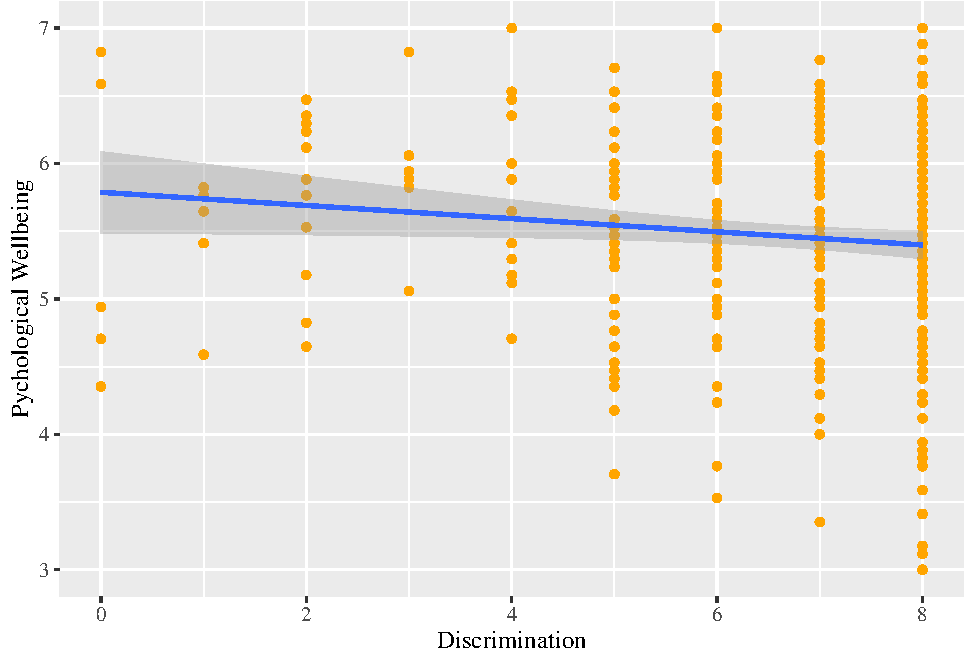
\includegraphics{prep_script_files/figure-latex/regplot-1.pdf}

We used R (Version 4.0.3; R Core Team, 2020) and the R-packages \emph{apaTables} (Version 2.0.5; Stanley, 2018), \emph{dplyr} (Version 1.0.2; Wickham, François, Henry, \& Müller, 2020), \emph{forcats} (Version 0.5.0; Wickham, 2019a), \emph{gdtools} (Version 0.2.2; Gohel, Wickham, Henry, \& Ooms, 2020), \emph{ggiraphExtra} (Version 0.3.0; Moon, 2020), \emph{ggplot2} (Version 3.3.2; Wickham, 2016), \emph{haven} (Version 2.3.1; Wickham \& Miller, 2020), \emph{janitor} (Version 2.0.1; Firke, 2020), \emph{knitr} (Version 1.30; Xie, 2015), \emph{lavaan} (Lishinski, 2018; Version 0.6.7; Rosseel, 2012), \emph{lavaanPlot} (Version 0.5.1; Lishinski, 2018), \emph{lm.beta} (Version 1.5.1; Behrendt, 2014), \emph{magick} (Version 2.5.2; Ooms, 2020), \emph{papaja} (Version 0.1.0.9997; Aust \& Barth, 2020), \emph{probemod} (Version 0.2.1; Tan, 2015), \emph{psych} (Version 2.0.9; Revelle, 2020), \emph{purrr} (Version 0.3.4; Henry \& Wickham, 2019), \emph{qwraps2} (Version 0.5.0; DeWitt, 2020), \emph{readr} (Version 1.3.1; Wickham, Hester, \& Francois, 2018), \emph{rio} (Version 0.5.16; Chan, Chan, Leeper, \& Becker, 2018), \emph{rockchalk} (Version 1.8.144; Johnson, 2019), \emph{stringr} (Version 1.4.0; Wickham, 2019b), \emph{tibble} (Version 3.0.4; Müller \& Wickham, 2020), \emph{tidyr} (Version 1.1.2; Wickham \& Henry, 2020), and \emph{tidyverse} (Version 1.3.0; Wickham et al., 2019) for all our analyses.

\hypertarget{results-1}{%
\section{Results}\label{results-1}}

\hypertarget{preliminary-analyses-1}{%
\subsection{Preliminary Analyses}\label{preliminary-analyses-1}}
=======
\hypertarget{procedure}{%
\subsection{Procedure}\label{procedure}}

For additional details on data collection procedures for Project STRIDE, please see Meyer, Frost, Narvaez, and Dietrich (2006).

\hypertarget{data-analysis}{%
\subsection{Data analysis}\label{data-analysis}}

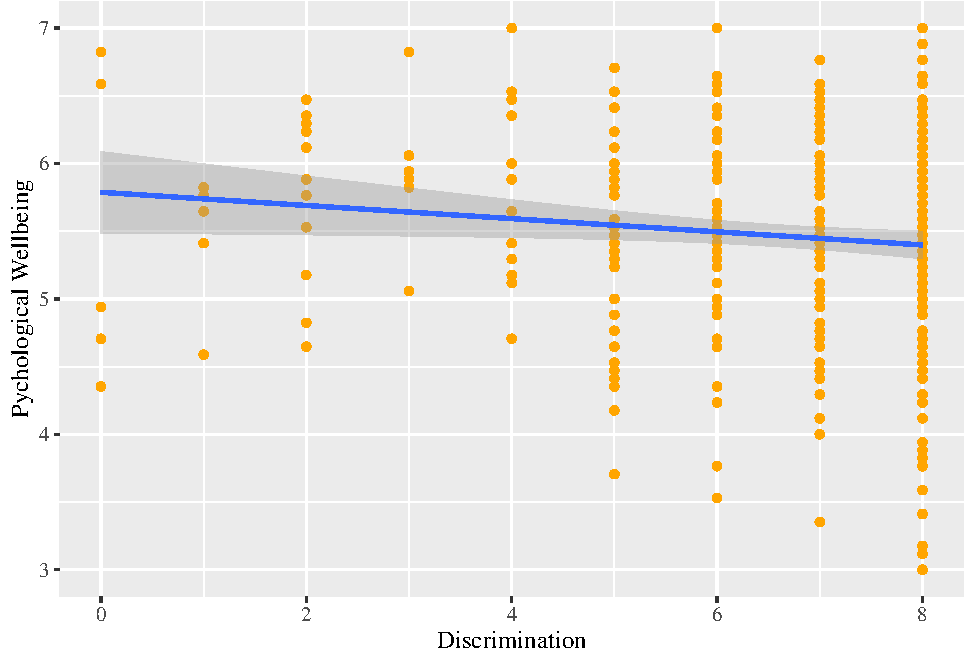
\includegraphics{prep_script_files/figure-latex/regplot-1.pdf}

We used R (Version 4.0.2; R Core Team, 2020) and the R-packages \emph{apaTables} (Version 2.0.5; Stanley, 2018), \emph{dplyr} (Version 1.0.2; Wickham, François, Henry, \& Müller, 2020), \emph{forcats} (Version 0.5.0; Wickham, 2019a), \emph{gdtools} (Version 0.2.2; Gohel, Wickham, Henry, \& Ooms, 2020), \emph{ggiraphExtra} (Version 0.3.0; Moon, 2020), \emph{ggplot2} (Version 3.3.2; Wickham, 2016), \emph{haven} (Version 2.3.1; Wickham \& Miller, 2020), \emph{janitor} (Version 2.0.1; Firke, 2020), \emph{knitr} (Version 1.30; Xie, 2015), \emph{lavaan} (Lishinski, 2018; Version 0.6.7; Rosseel, 2012), \emph{lavaanPlot} (Version 0.5.1; Lishinski, 2018), \emph{lm.beta} (Version 1.5.1; Behrendt, 2014), \emph{magick} (Version 2.5.2; Ooms, 2020), \emph{papaja} (Version 0.1.0.9997; Aust \& Barth, 2020), \emph{probemod} (Version 0.2.1; Tan, 2015), \emph{psych} (Version 2.0.9; Revelle, 2020), \emph{purrr} (Version 0.3.4; Henry \& Wickham, 2019), \emph{qwraps2} (Version 0.5.0; DeWitt, 2020), \emph{readr} (Version 1.4.0; Wickham, Hester, \& Francois, 2018), \emph{rio} (Version 0.5.16; Chan, Chan, Leeper, \& Becker, 2018), \emph{rockchalk} (Version 1.8.144; Johnson, 2019), \emph{stringr} (Version 1.4.0; Wickham, 2019b), \emph{tibble} (Version 3.0.4; Müller \& Wickham, 2020), \emph{tidyr} (Version 1.1.2; Wickham \& Henry, 2020), and \emph{tidyverse} (Version 1.3.0; Wickham et al., 2019) for all our analyses.

\hypertarget{results}{%
\section{Results}\label{results}}

\hypertarget{preliminary-analyses}{%
\subsection{Preliminary Analyses}\label{preliminary-analyses}}
>>>>>>> Stashed changes

Figure 1 displays the average number of everyday discriminatory experiences according to sexual orientation.

\begin{figure}

{\centering 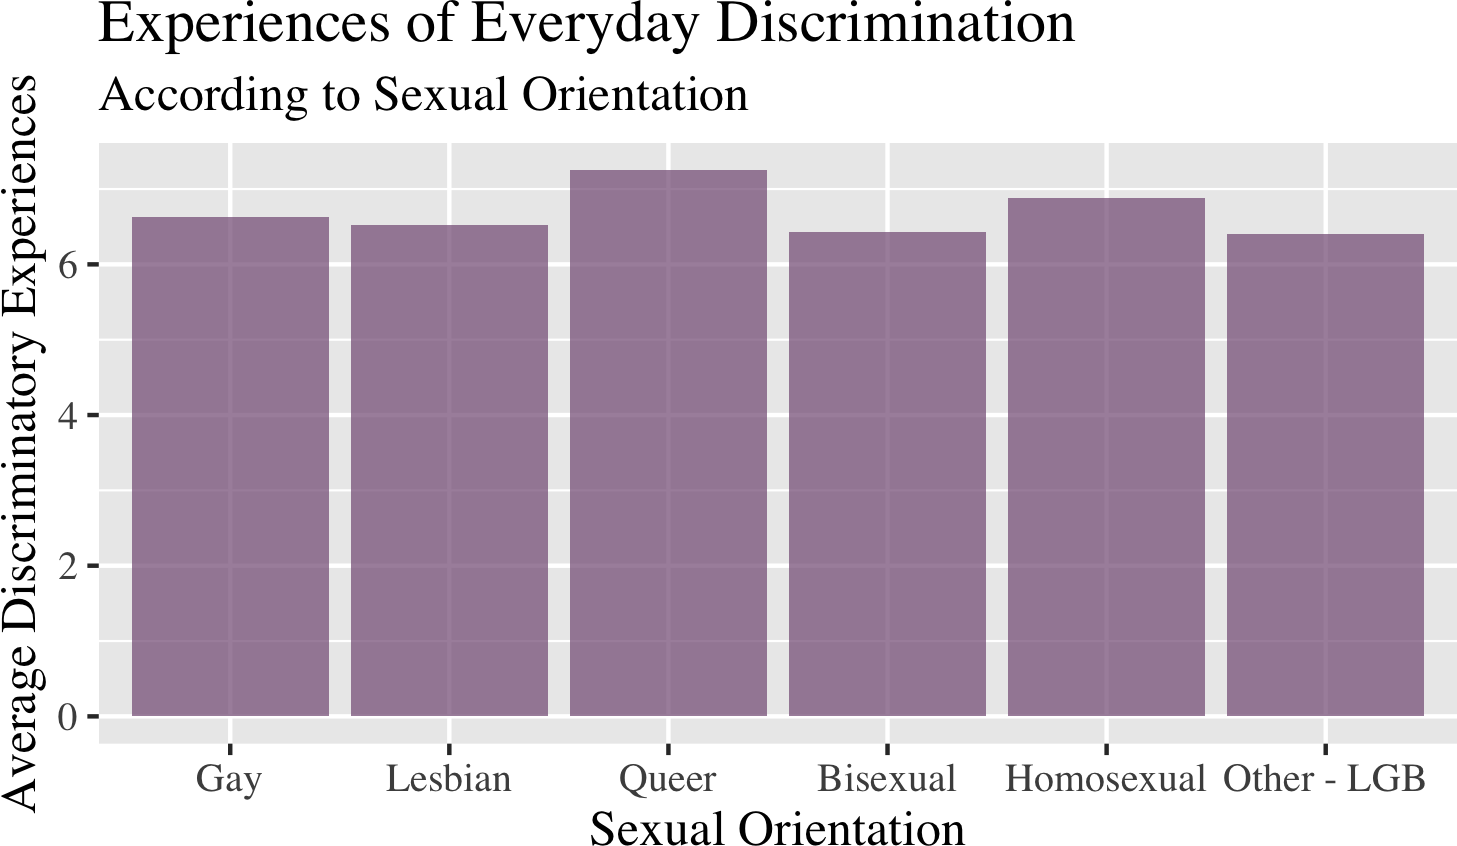
\includegraphics{prep_script_files/figure-latex/mean plot-1} 

}

\caption{Experiences of everyday discrimination according to sexual orientation.}(\#fig:mean plot)
\end{figure}

\begin{figure}

{\centering 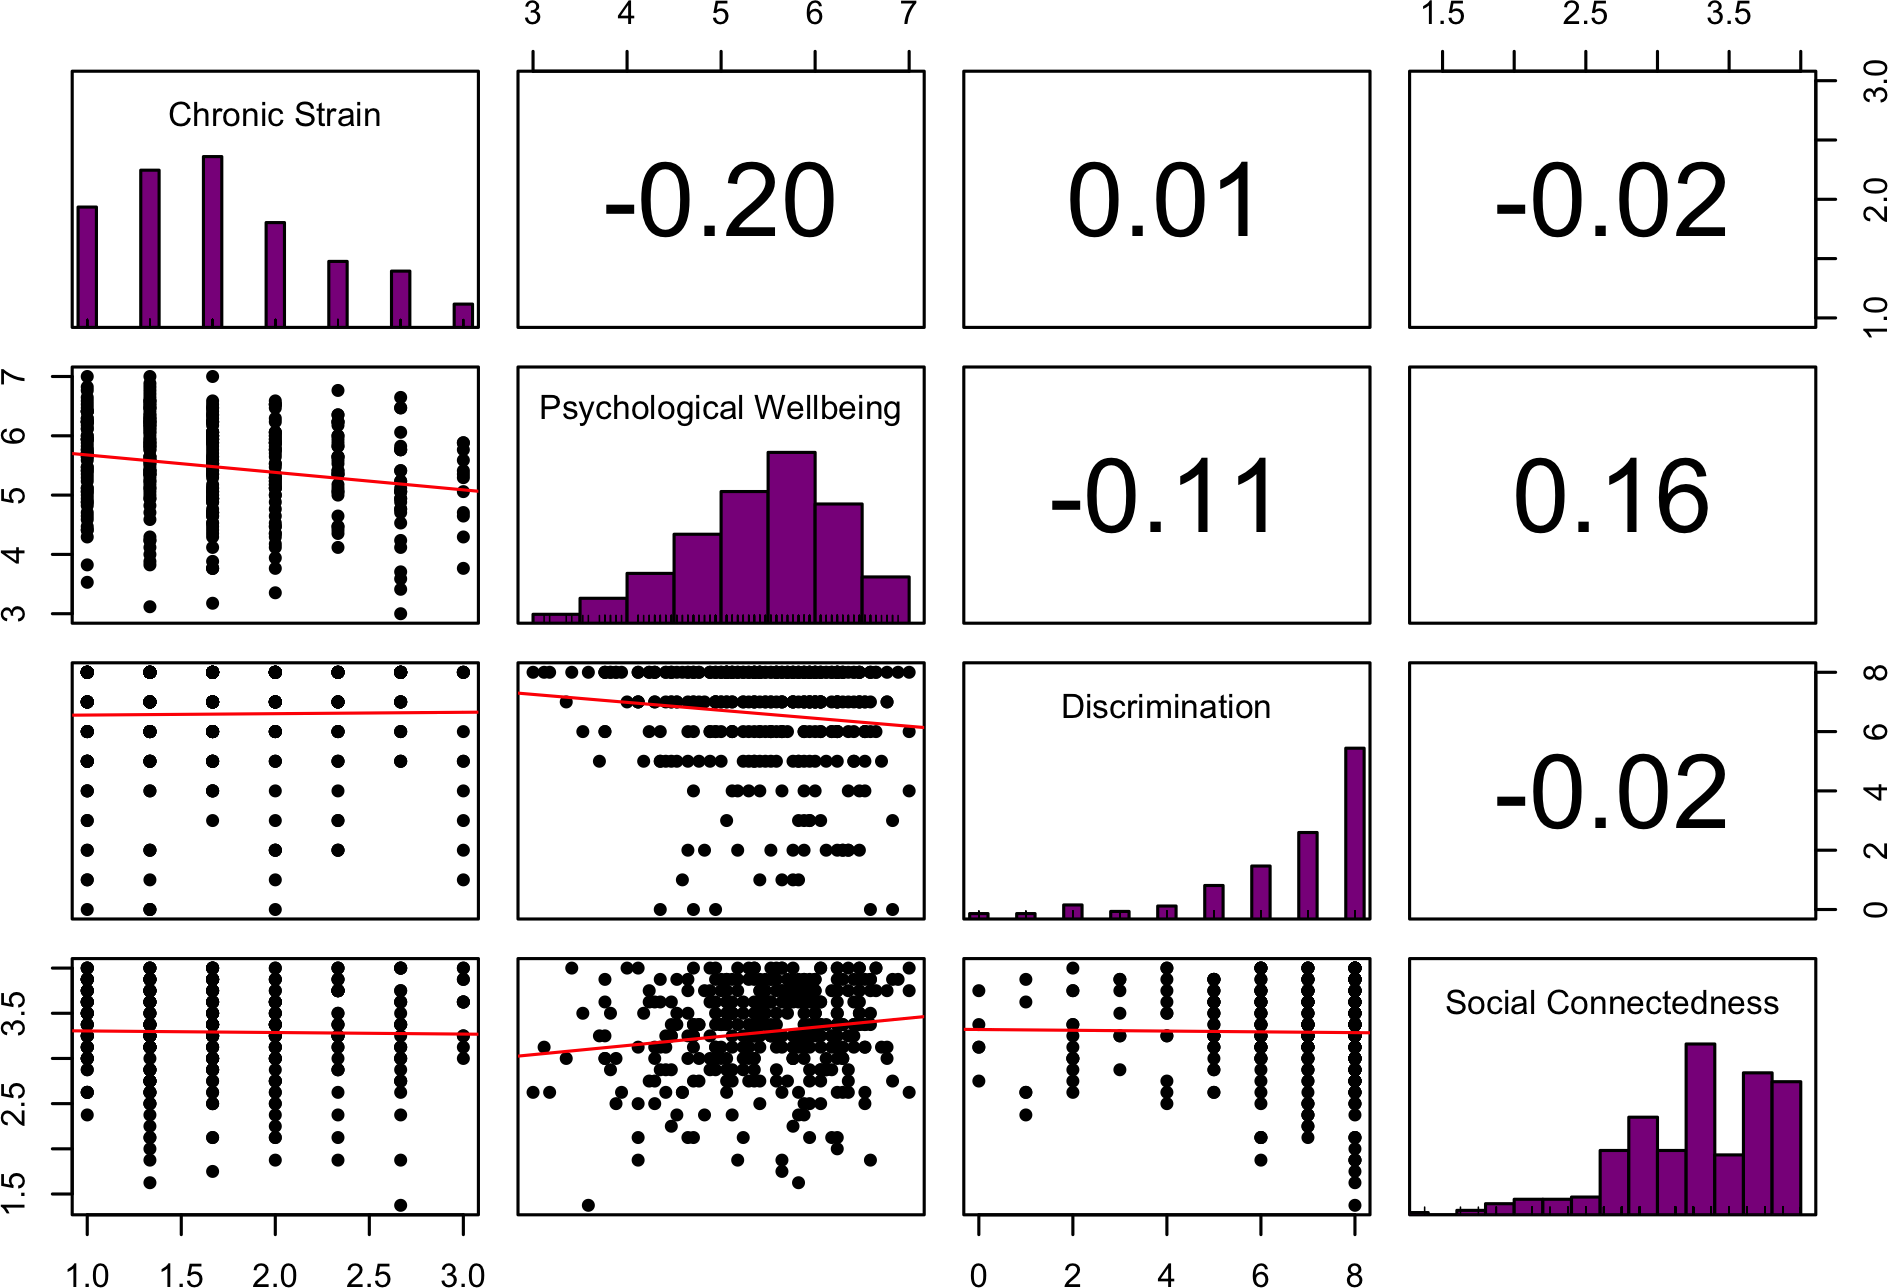
\includegraphics{prep_script_files/figure-latex/correlation panels-1} 

}

\caption{Correlation panels for all variables included in the model.}(\#fig:correlation panels)
\end{figure}

\begin{tabular}{l|r|r|r|r}
\hline
  & chr\_gen\_2 & perwellb\_2 & dis\_d\_total & connect\\
\hline
chr\_gen\_2 & 1.000 & -0.203 & 0.014 & -0.019\\
\hline
perwellb\_2 & -0.203 & 1.000 & -0.114 & 0.158\\
\hline
dis\_d\_total & 0.014 & -0.114 & 1.000 & -0.016\\
\hline
connect & -0.019 & 0.158 & -0.016 & 1.000\\
\hline
\end{tabular}

\hypertarget{primary-analyses}{%
\subsection{Primary Analyses}\label{primary-analyses}}

A multiple regression analysis was conducted to examine the effects of discriminatory experiences, chronic strain, social connectedness on psychological wellbeing among LGBQ individuals. When all variables were entered into the model, discriminatory experiences were negatively associated with psychological wellbeing, \(\hat{\beta_{1}}=-0.05, SE(\hat{\beta_{1}})=-0.11, t(356)=-2.14, p=.03\). Figure 3 displays the relationship between everday discrimination and psychological wellbeing. Likewise, consistent with hypothesis 2, chronic strain was significantly negatively associated with psychological wellbeing, \(\hat{\beta_{2}}=-0.29, SE(\hat{\beta_{2}})=-0.20, t(356)=-3.91, p < .001\). Consistent with hypothesis 3, social connectedness was significantly positively associated with psychological wellbeing, \(\hat{\beta_{3}}=0.24, SE(\hat{\beta_{3}})=0.15, t(356)=2.99, p < .001\). Taken together, all three predictors explained approximately 7.7\% of the variance in psychological wellbeing, \(F(3,356)=9.90, p<.001, R^{2}=.077\). Figure 4 displays the path model with corresponding beta coefficients.

\begin{figure}
<<<<<<< Updated upstream

{\centering 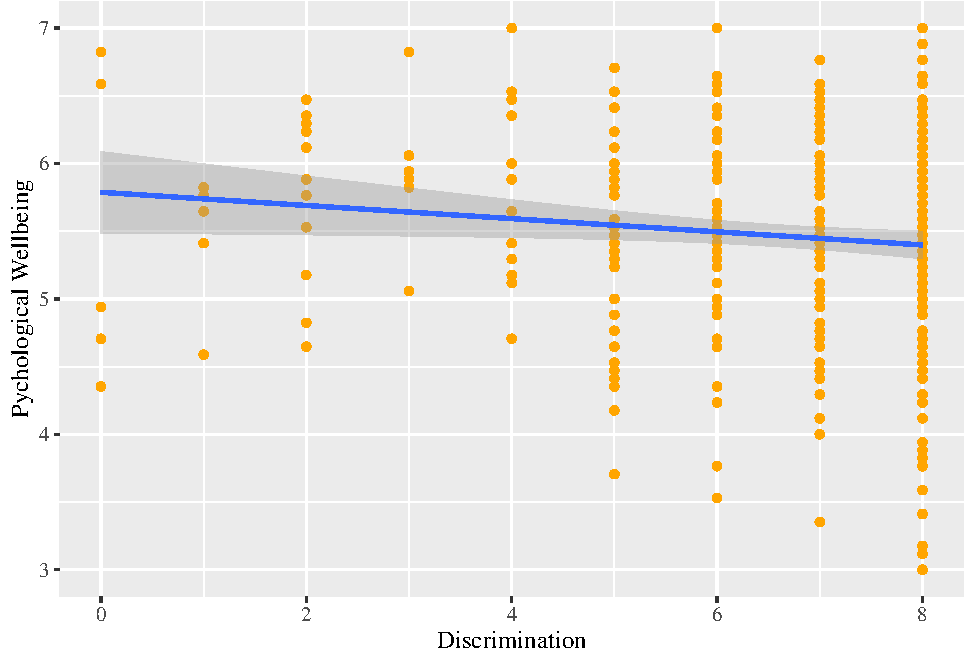
\includegraphics{prep_script_files/figure-latex/regression plot-1} 

}

\caption{Effect of everyday experiences of discrimination on psychological wellbeing in sexual minorities.}(\#fig:regression plot)
\end{figure}

\begin{figure}

{\centering 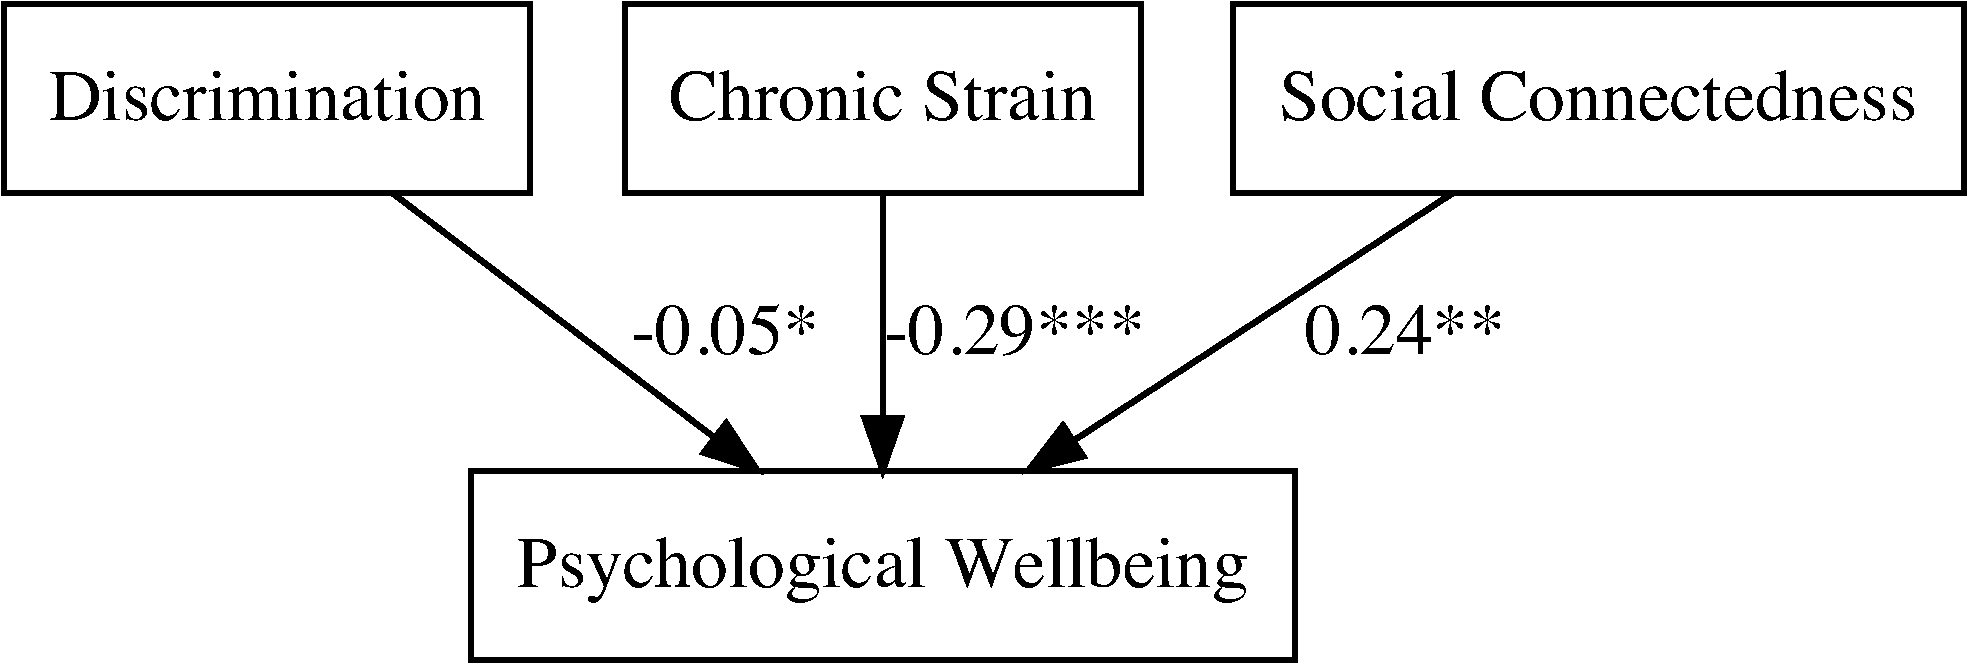
\includegraphics{prep_script_files/figure-latex/lavaan plot-1} 

}

=======

{\centering 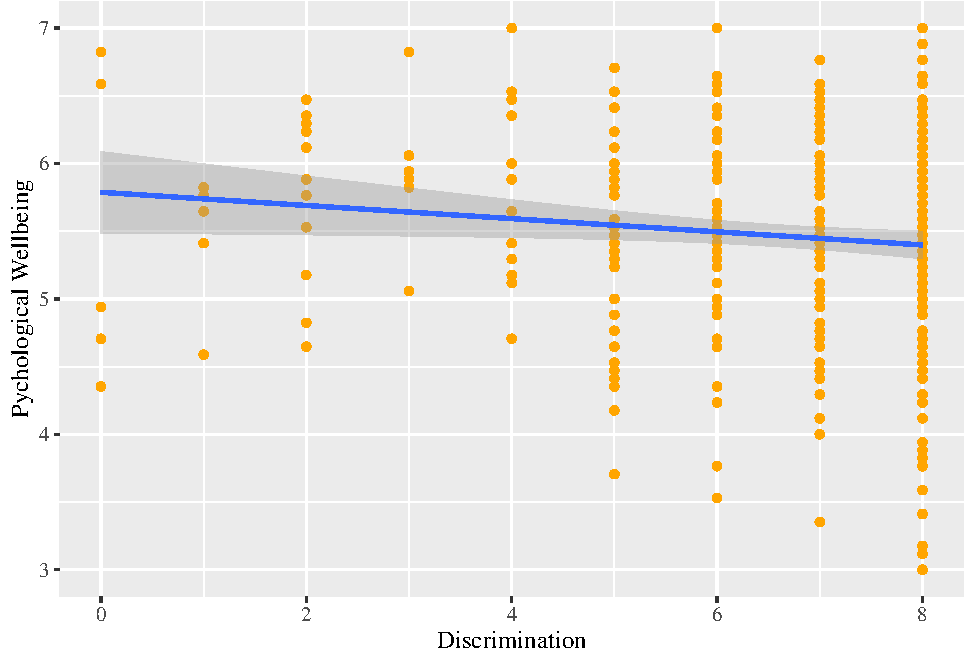
\includegraphics{prep_script_files/figure-latex/regression plot-1} 

}

\caption{Effect of everyday experiences of discrimination on psychological wellbeing in sexual minorities.}(\#fig:regression plot)
\end{figure}

\begin{figure}

{\centering 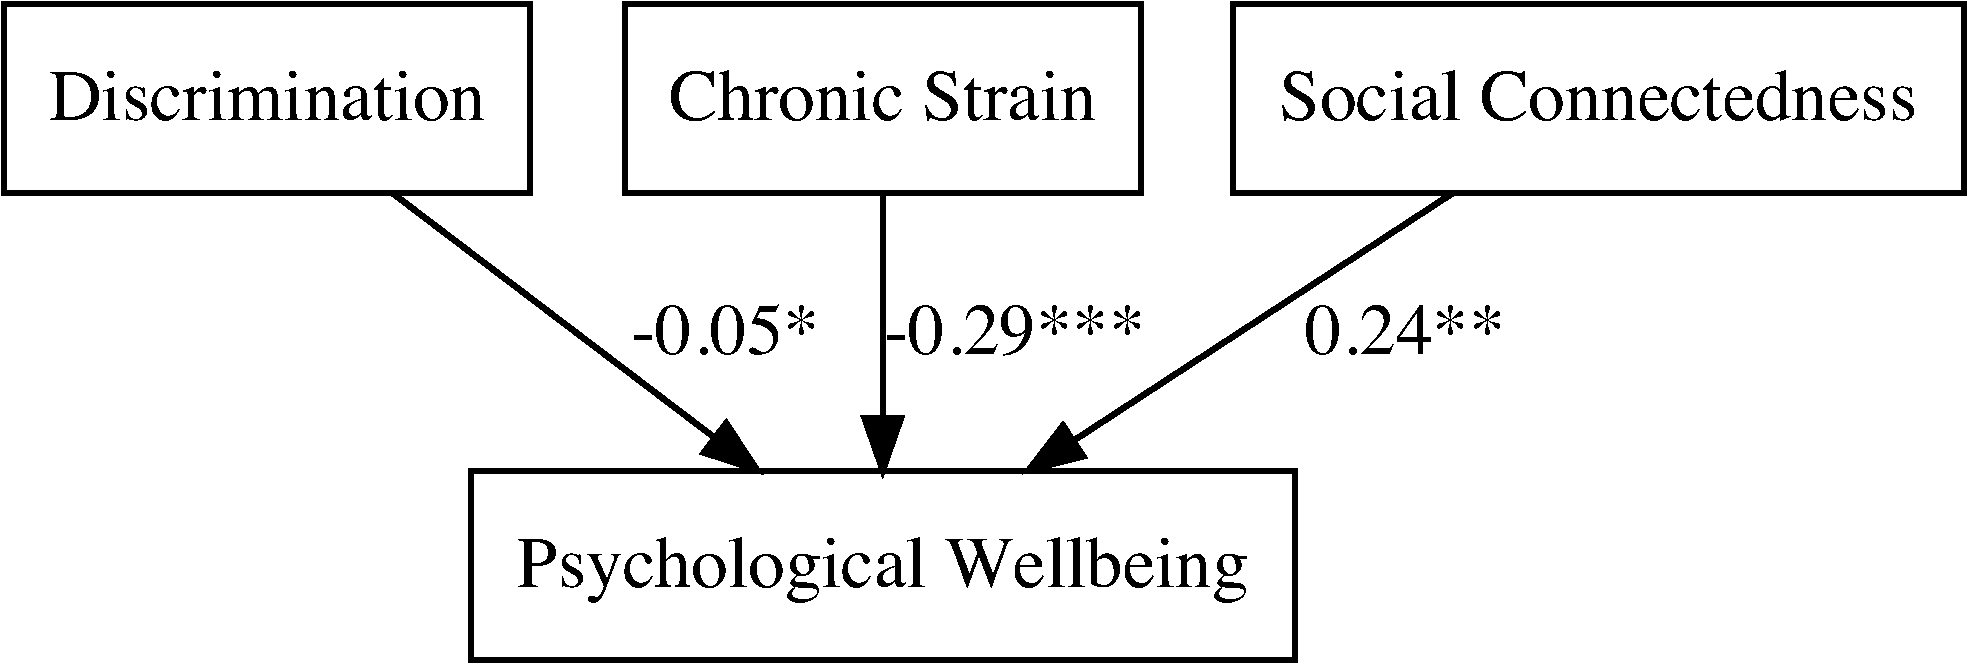
\includegraphics{prep_script_files/figure-latex/lavaan plot-1} 

}

>>>>>>> Stashed changes
\caption{Path model for the effect of discrimination, chronic strain, and social connectedness on psychological wellbeing.}(\#fig:lavaan plot)
\end{figure}

\hypertarget{discussion}{%
\section{Discussion}\label{discussion}}

\newpage

\hypertarget{references}{%
\section{References}\label{references}}

\begingroup
\setlength{\parindent}{-0.5in}
\setlength{\leftskip}{0.5in}

\hypertarget{refs}{}
\begin{CSLReferences}{1}{0}
\leavevmode\hypertarget{ref-R-papaja}{}%
Aust, F., \& Barth, M. (2020). \emph{{papaja}: {Create} {APA} manuscripts with {R Markdown}}. Retrieved from \url{https://github.com/crsh/papaja}

\leavevmode\hypertarget{ref-R-lm.beta}{}%
Behrendt, S. (2014). \emph{Lm.beta: Add standardized regression coefficients to lm-objects}. Retrieved from \url{https://CRAN.R-project.org/package=lm.beta}

\leavevmode\hypertarget{ref-R-rio}{}%
Chan, C., Chan, G. C., Leeper, T. J., \& Becker, J. (2018). \emph{Rio: A swiss-army knife for data file i/o}.

\leavevmode\hypertarget{ref-R-qwraps2}{}%
DeWitt, P. (2020). \emph{qwraps2: Quick wraps 2}. Retrieved from \url{https://CRAN.R-project.org/package=qwraps2}

\leavevmode\hypertarget{ref-R-janitor}{}%
Firke, S. (2020). \emph{Janitor: Simple tools for examining and cleaning dirty data}. Retrieved from \url{https://CRAN.R-project.org/package=janitor}

\leavevmode\hypertarget{ref-R-gdtools}{}%
Gohel, D., Wickham, H., Henry, L., \& Ooms, J. (2020). \emph{Gdtools: Utilities for graphical rendering}. Retrieved from \url{https://CRAN.R-project.org/package=gdtools}

\leavevmode\hypertarget{ref-R-purrr}{}%
Henry, L., \& Wickham, H. (2019). \emph{Purrr: Functional programming tools}. Retrieved from \url{https://CRAN.R-project.org/package=purrr}

\leavevmode\hypertarget{ref-R-rockchalk}{}%
Johnson, P. E. (2019). \emph{Rockchalk: Regression estimation and presentation}. Retrieved from \url{https://CRAN.R-project.org/package=rockchalk}

\leavevmode\hypertarget{ref-R-lavaanPlot}{}%
Lishinski, A. (2018). \emph{lavaanPlot: Path diagrams for lavaan models via DiagrammeR}. Retrieved from \url{https://CRAN.R-project.org/package=lavaanPlot}

\leavevmode\hypertarget{ref-projectstride}{}%
Meyer, I. H., Dohrenwend, B. P., Schwartz, S., Hunter, J., \& Kertzner, R. M. (2016). Project STRIDE: Stress, identity, and mental health, new york city, 2004-2005: Version 2. Inter-University Consortium for Political; Social Research. \url{https://doi.org/10.3886/ICPSR35525.V2}

\leavevmode\hypertarget{ref-projectstridemethod}{}%
Meyer, I. H., Frost, D. M., Narvaez, R., \& Dietrich, J. H. (2006). Project stride methodology and technical notes. \emph{Unpublished Manuscript}.

\leavevmode\hypertarget{ref-mills2001}{}%
Mills, T. C., Stall, R., Pollack, L., Paul, J. P., Binson, D., Canchola, J., \& Catania, J. A. (2001). Health-related characteristics of men who have sex with men: A comparison of those living in" gay ghettos" with those living elsewhere. \emph{American Journal of Public Health}, \emph{91}(6), 980.

\leavevmode\hypertarget{ref-R-ggiraphExtra}{}%
Moon, K.-W. (2020). \emph{ggiraphExtra: Make interactive 'ggplot2'. Extension to 'ggplot2' and 'ggiraph'}. Retrieved from \url{https://CRAN.R-project.org/package=ggiraphExtra}

\leavevmode\hypertarget{ref-R-tibble}{}%
Müller, K., \& Wickham, H. (2020). \emph{Tibble: Simple data frames}. Retrieved from \url{https://CRAN.R-project.org/package=tibble}

\leavevmode\hypertarget{ref-R-magick}{}%
Ooms, J. (2020). \emph{Magick: Advanced graphics and image-processing in r}. Retrieved from \url{https://CRAN.R-project.org/package=magick}

\leavevmode\hypertarget{ref-R-base}{}%
R Core Team. (2020). \emph{R: A language and environment for statistical computing}. Vienna, Austria: R Foundation for Statistical Computing. Retrieved from \url{https://www.R-project.org/}

\leavevmode\hypertarget{ref-R-psych}{}%
Revelle, W. (2020). \emph{Psych: Procedures for psychological, psychometric, and personality research}. Evanston, Illinois: Northwestern University. Retrieved from \url{https://CRAN.R-project.org/package=psych}

\leavevmode\hypertarget{ref-R-lavaan}{}%
Rosseel, Y. (2012). {lavaan}: An {R} package for structural equation modeling. \emph{Journal of Statistical Software}, \emph{48}(2), 1--36. Retrieved from \url{http://www.jstatsoft.org/v48/i02/}

\leavevmode\hypertarget{ref-ryff1989}{}%
Ryff, C. D. (1989). Happiness is everything, or is it? Explorations on the meaning of psychological well-being. \emph{Journal of Personality and Social Psychology}, \emph{57}(6), 1069.

\leavevmode\hypertarget{ref-ryffkeyes1995}{}%
Ryff, C. D., \& Keyes, C. L. M. (1995). The structure of psychological well-being revisited. \emph{Journal of Personality and Social Psychology}, \emph{69}(4), 719.

\leavevmode\hypertarget{ref-R-apaTables}{}%
Stanley, D. (2018). \emph{apaTables: Create american psychological association (APA) style tables}. Retrieved from \url{https://CRAN.R-project.org/package=apaTables}

\leavevmode\hypertarget{ref-R-probemod}{}%
Tan, J. C. (2015). \emph{Probemod: Statistical tools for probing moderation effects}. Retrieved from \url{https://CRAN.R-project.org/package=probemod}

\leavevmode\hypertarget{ref-wheaton1999}{}%
Wheaton, B. (1999). The nature of stressors. In A. F. Horwitz \& T. L. Scheid (Eds.), \emph{A handbook for the study of mental health: Social contexts, theories, and systems} (pp. 176--197). New York: Oxford University Press.

\leavevmode\hypertarget{ref-R-ggplot2}{}%
Wickham, H. (2016). \emph{ggplot2: Elegant graphics for data analysis}. Springer-Verlag New York. Retrieved from \url{https://ggplot2.tidyverse.org}

\leavevmode\hypertarget{ref-R-forcats}{}%
Wickham, H. (2019a). \emph{Forcats: Tools for working with categorical variables (factors)}. Retrieved from \url{https://CRAN.R-project.org/package=forcats}

\leavevmode\hypertarget{ref-R-stringr}{}%
Wickham, H. (2019b). \emph{Stringr: Simple, consistent wrappers for common string operations}. Retrieved from \url{https://CRAN.R-project.org/package=stringr}

\leavevmode\hypertarget{ref-R-tidyverse}{}%
Wickham, H., Averick, M., Bryan, J., Chang, W., McGowan, L. D., François, R., \ldots{} Yutani, H. (2019). Welcome to the {tidyverse}. \emph{Journal of Open Source Software}, \emph{4}(43), 1686. \url{https://doi.org/10.21105/joss.01686}

\leavevmode\hypertarget{ref-R-dplyr}{}%
Wickham, H., François, R., Henry, L., \& Müller, K. (2020). \emph{Dplyr: A grammar of data manipulation}. Retrieved from \url{https://CRAN.R-project.org/package=dplyr}

\leavevmode\hypertarget{ref-R-tidyr}{}%
Wickham, H., \& Henry, L. (2020). \emph{Tidyr: Tidy messy data}. Retrieved from \url{https://CRAN.R-project.org/package=tidyr}

\leavevmode\hypertarget{ref-R-readr}{}%
Wickham, H., Hester, J., \& Francois, R. (2018). \emph{Readr: Read rectangular text data}. Retrieved from \url{https://CRAN.R-project.org/package=readr}

\leavevmode\hypertarget{ref-R-haven}{}%
Wickham, H., \& Miller, E. (2020). \emph{Haven: Import and export 'SPSS', 'stata' and 'SAS' files}. Retrieved from \url{https://CRAN.R-project.org/package=haven}

\leavevmode\hypertarget{ref-williams1997}{}%
Williams, D. R., Yu, Y., Jackson, J. S., \& Anderson, N. B. (1997). Racial differences in physical and mental health: Socio-economic status, stress and discrimination. \emph{Journal of Health Psychology}, \emph{2}(3), 335--351.

\leavevmode\hypertarget{ref-R-knitr}{}%
Xie, Y. (2015). \emph{Dynamic documents with {R} and knitr} (2nd ed.). Boca Raton, Florida: Chapman; Hall/CRC. Retrieved from \url{https://yihui.org/knitr/}

\end{CSLReferences}

\endgroup


\end{document}
